\documentclass[11pt,english,a4paper]{report}

\usepackage[toc,xindy]{glossaries} 
\usepackage{graphicx} % Displaying pictures in the document.
\usepackage[floatrow]{chemstyle} % Displaying figures next to item lists.
\usepackage[hidelinks]{hyperref}
\usepackage{listings} % Adding source code listings.
\usepackage{color}


\definecolor{mygreen}{rgb}{0,0.6,0}
\definecolor{mygray}{rgb}{0.5,0.5,0.5}
\definecolor{mymauve}{rgb}{0.58,0,0.82}

\lstset{ %
  backgroundcolor=\color{white},   % choose the background color; you must add \usepackage{color} or \usepackage{xcolor}
  basicstyle=\footnotesize,        % the size of the fonts that are used for the code
  breakatwhitespace=false,         % sets if automatic breaks should only happen at whitespace
  breaklines=true,                 % sets automatic line breaking
  captionpos=b,                    % sets the caption-position to bottom
  commentstyle=\color{mygreen},    % comment style
  deletekeywords={...},            % if you want to delete keywords from the given language
  escapeinside={\%*}{*)},          % if you want to add LaTeX within your code
  extendedchars=true,              % lets you use non-ASCII characters; for 8-bits encodings only, does not work with UTF-8
  frame=single,                    % adds a frame around the code
  keepspaces=true,                 % keeps spaces in text, useful for keeping indentation of code (possibly needs columns=flexible)
  keywordstyle=\color{blue},       % keyword style
  language=Octave,                 % the language of the code
  morekeywords={public, if, for, else, class, import, return, null},            % if you want to add more keywords to the set
  numbers=left,                    % where to put the line-numbers; possible values are (none, left, right)
  numbersep=5pt,                   % how far the line-numbers are from the code
  numberstyle=\tiny\color{mygray}, % the style that is used for the line-numbers
  rulecolor=\color{black},         % if not set, the frame-color may be changed on line-breaks within not-black text (e.g. comments (green here))
  showspaces=false,                % show spaces everywhere adding particular underscores; it overrides 'showstringspaces'
  showstringspaces=false,          % underline spaces within strings only
  showtabs=false,                  % show tabs within strings adding particular underscores
  stepnumber=1,                    % the step between two line-numbers. If it's 1, each line will be numbered
  stringstyle=\color{mymauve},     % string literal style
  tabsize=2,                       % sets default tabsize to 2 spaces
  title=\lstname                   % show the filename of files included with \lstinputlisting; also try caption instead of title
}


\title{INF226 - Project Report}
\date{\today}
\author{Lasse K. Brun - lkbrun@gmail.com \\ Havard R. Olsen - haavard.olsen@live.com}


\newglossaryentry{js} 		{ name=JavaScript,	description={A scripting language used in web development}}
\newglossaryentry{java}		{ name=Java,		description={A programming language }}
\newglossaryentry{maven}	{ name=Maven,		description={A software project management and comprehension tool }}


\newacronym{svn}{SVN}{Subversion}
\newacronym{uib}{UiB}{University of Bergen}
\newacronym{zap}{ZAP}{OWASP Zed Attack Proxy}
\newacronym{for}{FOR}{HP Fortify}
\newacronym{gis}{GIS}{Geographic Information System}
\newacronym{sca}{SCA}{Static Code Analyser}
\newacronym{url}{URL}{Uniform Resource Locator}
\newacronym{jre}{JRE}{Java Runtime Environment}
\newacronym{xss}{XSS}{Cross Site Scripting}

\newacronym{http}{HTTP}{Hypertext Transfer Protocol}
\newacronym{dhis}{DHIS 2}{District Health Information System 2}

\newacronym{regex}{REGEX}{Regular Expression}
\newacronym{owasp}{OWASP}{Open Web Application Security Project}



 
\makeglossaries

\begin{document}

\maketitle

\tableofcontents
\newpage

% List of figures
\listoffigures
\newpage

% Glossary
\printglossaries
\newpage


\chapter{Introduction}
\textit{This chapter will provide you with some background material for the report, why we are writing it and what we hope to accomplish.}

\section{Motivation}
\paragraph{}
Security is more important than ever in today's software world. 
New and refined attack methods keep emerging, making creation of secure software applications a full time job. 
This has caused production of new, innovative tools and frameworks to handle analysis of software. 
The tools and frameworks help software developers to find security breaches within their application. 
Throughout this report will two common tools be introduced, and tested on an actual codebase.

\paragraph{}
We will be using the \gls{dhis} as codebase. \gls{dhis} is a flexible, web-based open-source information system. 
The system has visualization features such as \gls{gis}, charts and pivot tables. You can read more about the system on their website \cite{dhis2-homepage}.


\section{Goal}
\paragraph{}
The goal of this report is to expose security breaches within the codebase(\gls{dhis}). 
This will give us a better understanding of how the analysing tools work and how to use them. 
Thereafter will we provide an evaluation based on the result given by the tools. 
The evaluation will result in a conclusion, centred around a solution to the security flaws. 
Giving this report to the company responsible for the codebase, will hopefully give them an understanding of the security holes in their application and a solution to how they can resolve them.

\chapter{Installation of tools and code base}
\label{cha:part2}
\textit{In this chapter will more concise details about the two tools be described, and go deeper into the provided codebase.}

\section{OWASP Zed Attack Proxy}
\paragraph{}
\gls{zap} is an integrated penetration testing tool used for finding flaws and vulnerabilities in web applications. 
\gls{zap} is an excellent tool for both beginners and security experts as it provides an easy to use graphical interface as well as a more in-depth command line.

\paragraph{}
This section will cover some of the features that \gls{zap} provides, and see how it can be beneficial.

\subsection{Installation and Experience}
The installation process is relatively straight forward as you are guided through an installation wizard. 
This is sufficient enough for basic usage. 
On the other hand, for more advanced usage you will need to do some additional configuration. 
This includes setting up \glspl{zap} intercepting proxy and running different kinds of scans. 
The \gls{zap} home page has multiple tutorials and plenty of documentation on how to use different features found in \gls{zap}. 
These features will be discussed further in the next section.

\subsection{Features}
\subsubsection{Intercepting proxy}
\gls{zap} is actually an intercepting proxy which is capable of intercepting requests and responses.
This means that you can read the traffic as well as change them.
This can be utilized by configuring your browser to use \gls{zap} as a proxy.
As a result can you optimize the analysis by doing manual testing of the application before you run any active scan or spider.

\begin{figure}[h]
    \centering
    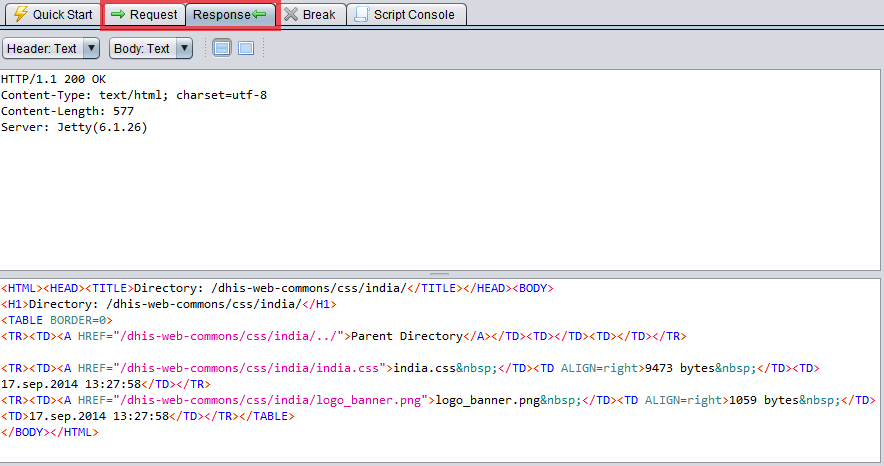
\includegraphics[scale=0.45]{images/zap-right-menu.png}
    \caption{Example of monitoring the network traffic. }
    \label{fig:zaprightmenu}
\end{figure}

\subsubsection{Passive and Active scanner}
The documentation for \gls{zap} states that you should only use \gls{zap} on applications you have permission to do so, as you are actually attacking the application. 
This does not include the passive scanner. 
This is a tool that will run in the background as you browse the application, only listening to the network traffic and not attacking.

\paragraph{}
\gls{zap} also includes an active scanner, which unlike the passive scanner will perform various attacks on the application. 
It is worth noting that the active scanner can only find certain kinds of vulnerabilities. 
So to fully utilize \gls{zap}, you should do manual penetration testing as well as run the active scan.

\begin{figure}[h]
    \centering
    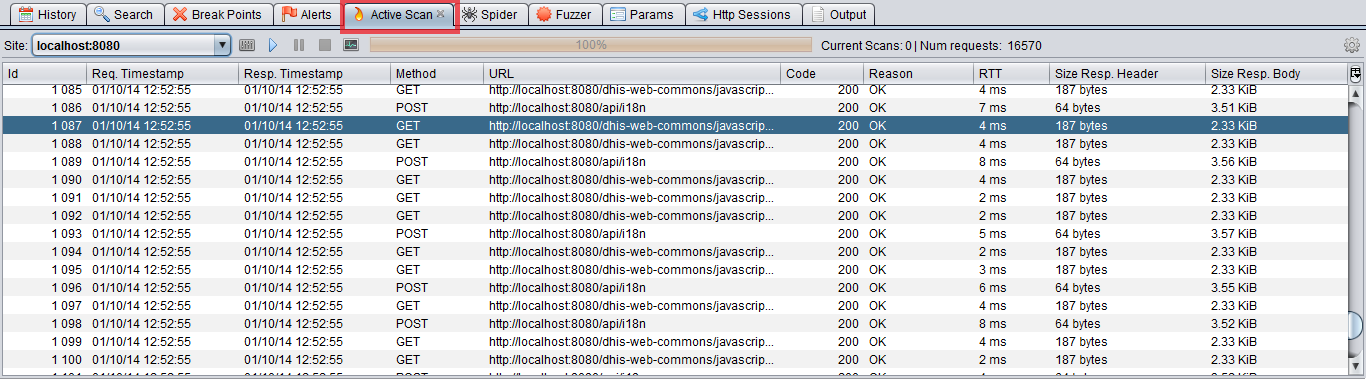
\includegraphics[scale=0.35]{images/zap-active-scan.png}
    \caption{Result of running an active scan. }
    \label{fig:zapactivescan}
\end{figure}

\subsubsection{Spider}
\gls{zap} comes with a built in spider which crawls the application looking for \glspl{url}.
It starts of with the initial list. 
Then it visits all \glspl{url} on the list and finds the \gls{url} resources on each page. 
The spider doesn't stop until it has visited every hyperlink in the application.
The spider will find resources that you may have missed during penetration testing or that has been hidden from you. 
It is a great tool to make sure that you cover the entire application.

\begin{figure}[h]
    \centering
    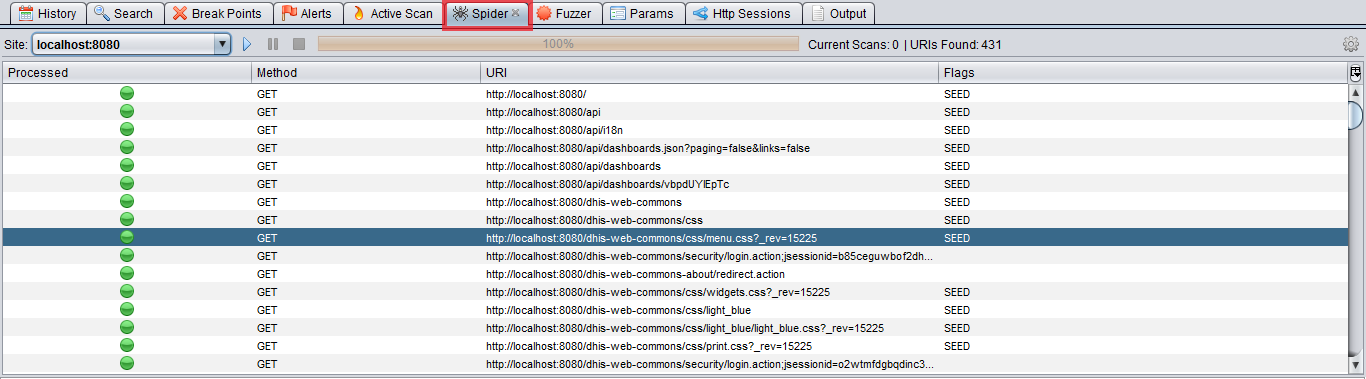
\includegraphics[scale=0.35]{images/zap-spider.png}
    \caption{Result of running the spider. }
    \label{fig:zapspider}
\end{figure}

\subsection{Summary}
\paragraph{}
\gls{zap} is great tool with many helpful features, but that doesn't mean that you can rely solely on the automatic scanners it provides. 
By using \gls{zap} together with manual penetration testing can you achieve the best result and the best coverage. 
Figure~\ref{fig:zapscreenshot}  shows the result of running \gls{zap} on the \gls{dhis} application. You can read more about \gls{zap} here. \cite{zap-documentation,zap-homepage}


\begin{figure}[h]
    \centering
    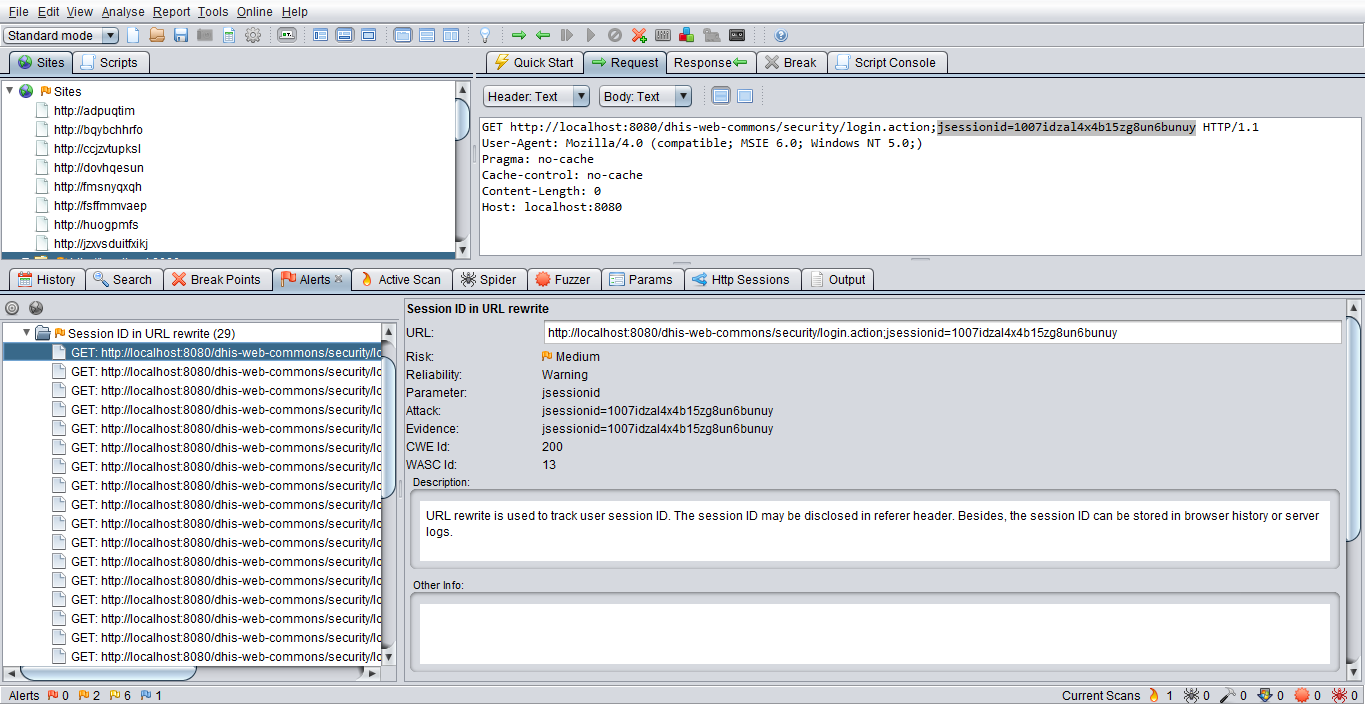
\includegraphics[scale=0.35]{images/zap-sc.png}
    \caption{Screenshot of running \gls{zap} on the codebase}
    \label{fig:zapscreenshot}
\end{figure}


\newpage

\section{HP Fortify}
\label{sectionfortifytool}
\paragraph{}
HP Fortify assess, assure and protect enterprise software and applications from security vulnerabilities.
Providing complete security testing and management through static and dynamic testing technologies. 
Or, by repeatable and auditable secure behaviours, over the course of a software application life cycle. 
A flexible delivery model allows security groups to get started quickly and scale in response to business changes while protecting their assets in application security. 
You can read more about HP Fortify here. \cite{fortify-software-wiki, fortify-software-homepage-features} 

\subsection{Installation and Experience}
\paragraph{}
Installing the HP Fortify plug in for Eclipse is a straightforward process. 
First of all, must the HP Fortify software be downloaded and installed.
\gls{uib} provided access to their \gls{svn} repository where the HP Fortify software tool could be downloaded.  
The download includes an installation wizard. 
The default installation covers our needs for this project, however, you can specify specific configurations throughout the wizard. \cite{installation-usage-guide}

\paragraph{}
There exists a HP Fortify plug-in for Eclipse which is easy and convenient to use.
Eclipse has a feature called install new software, where a wizard will take you through the plug-in installation steps.
There you have to specify the installation directory of HP Fortify meaning the HP Fortify software you installed in the previous step.
Here you will have some different configuration settings, for instance what features to install.
After completion of the installation, a simple restart of Eclipse is needed and the menu bar will then include the HP Fortify menu shown in Figure~\ref{fig:fortifymenuscreenshot}. \cite{installation-usage-guide}

\begin{figure}[h]
    \centering
    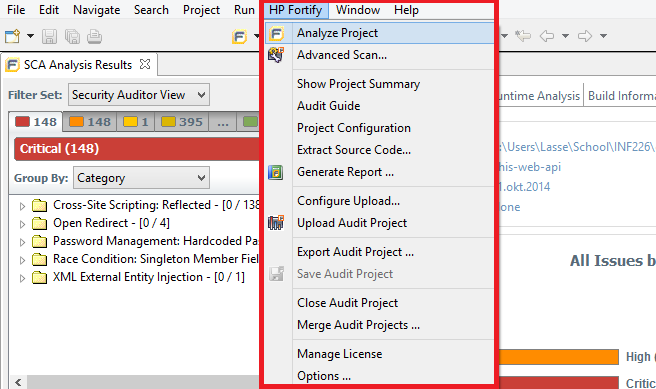
\includegraphics[scale=0.45]{images/fortifymenu-sc.png}
    \caption{After the installation and restart of Eclipse will the HP Fortify menu show in the menu bar of Eclipse.}
    \label{fig:fortifymenuscreenshot}
\end{figure}

\subsection{Features}
\paragraph{}
The plug-in consists of two components: an audit plug-in component and an analysis plug-in component. 
The audit plug-in makes it possible to open and audit former scan results and audit them. 
The analysis plug-in enables you to initiate a \gls{sca} scan and analysis, view the result and fix the discovered security flaws. \cite{installation-usage-guide}

\subsubsection{HP Fortify \gls{sca}}
\paragraph{}
This component makes it possible to initiate a \gls{sca} scan and analysis of your \gls{java} source code.
You can scan entire projects or specify a single package or file that you want to scan. 
Although the plug-in automatically includes all source files from dependencies. 
A scan can easily be started by selecting the desired project, package or file and start the scan from the HP Fortify menu.
The result of the scan will be shown in a new tab in Eclipse, called the \gls{sca} Analysis Result view. \cite{installation-usage-guide}

\paragraph{}
The \gls{sca} Analysis Result view provides a way to group and select security issues that you want to audit. 
Within the view you can set a filter which specifies what issues should be shown, and how they should be listed.
There are many different ways to show the result.
You can for instance choose between Security Auditor View, Developer View, Critical Exposure and Hotspot.

\begin{figure}[h]
    \centering
    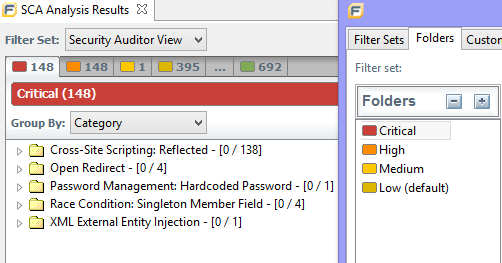
\includegraphics[scale=0.65]{images/fortifyfolders-sc.png}
    \caption{Showing the different color codes for folders. Critical, High, Medium and Low. }
    \label{fig:fortifyfoldersscreenshot}
\end{figure}

\paragraph{}
The issues are sorted by severity, and put into folders accordingly such as critical, high, medium and low. 
When you select an issue, the Analyse Evidence view will be displayed. \cite{installation-usage-guide}

\paragraph{}
\label{analyseevidence}
The Analyse Evidence view presents a justification for why this is an issue.
The view will give a more detailed reason for why this is an issue, and show the direction of the data flow and how the data flow moves. \cite{installation-usage-guide}

\paragraph{}
The Project Summary view displays detailed scan information in different tabs.

\begin{figure}[h]
    \centering
    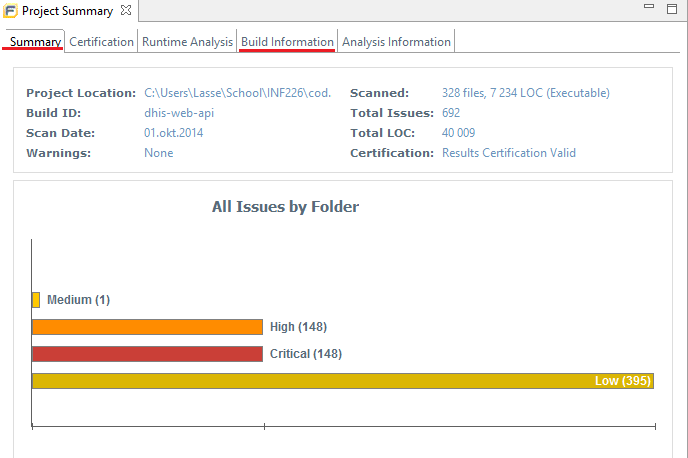
\includegraphics[scale=0.65]{images/fortifysummary-sc.png}
    \caption{Project summary of running a \gls{sca} scan on the codebase. You can switch between different tabs at the top. }
    \label{fig:fortifysummaryscreenshot}
\end{figure}

For instance, a summary tab displaying high-level information about the project and a build information tab showing build id, number of files scanned, date of scan and more applicable information about the scan and project. \cite{installation-usage-guide}

\subsubsection{Auditing Analysis Results}
\paragraph{}
This component is responsible for auditing and analysis of the result.
It is possible to open an existing audit and continue your work.
You can even open the analysis for a project created by someone else on another machine.
If necessary, can you generate a new result from the audit. \cite{installation-usage-guide}

\paragraph{}
The Analysis Evidence view is mentioned in Section~\ref{analyseevidence}. 
It is possible to display the Analyse Evidence view here as well which gives a more detailed reason of a particular issue.
In addition, can you do various of search queries that can contain, be equal/not equal to a text.
You can use \gls{regex} or search for number range and even more. 
Finally can you generate a report based on the analysis data that will show the result of analysis. \cite{installation-usage-guide}


\section{\gls{dhis}}
\paragraph{}
The system is very widespread being the preferred health management information system in 46 countries across five continents. 
The health system helps governments and health organizations to manage their operations more efficiently, monitor processes and improve communication. 
The system is portable and can capture data on any type of device, including desktops, laptops, tablets and smartphones. 

\paragraph{}
The system is basically a routine data based health information system. 
The system has a three-layered architecture and is written in \gls{java} as shown in~\ref{fig:dhisarch}.
The presentation layer is web-based, and the system can be used online as well as standalone.
The business layer holds most of the application logic and provides methods that delegate to a corresponding method in the persistence layer.
The persistence layer is based on Hibernate, which allows the application to run on any major \gls{dbms}.
More information about the system can be found here \cite{dhis2-homepage, dhis2-wiki}.

\begin{figure}[h]
    \centering
    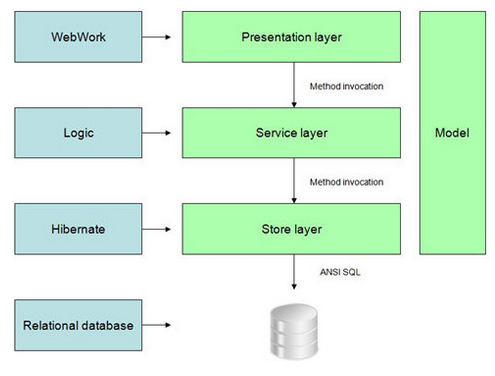
\includegraphics[scale=0.65]{images/dhis2-architecture.png}
    \caption{Diagram displaying the architecture of the \gls{dhis} application. }
    \label{fig:dhisarch}
\end{figure}


\subsection{Installation and Experience}
\paragraph{}
After following the installation guideline for the codebase found at their homepage, we learned that the information there was insufficient.
It explains how to use \gls{maven} to build the different components and how to set up the database connection, but this only took us so far.
First of all we had to add a new environment variable which specified the location of the database configuration file.
After this, the build was successful, but running the application failed due an OutOfMemoryException. 
This means that the web server didn't have access to enough memory to successfully run the application. 
We fixed this by adding two more environment variables which specified the allocated memory for the \gls{jre} and for \gls{maven}.
Finally the application ran successfully and the project could be built as an Eclipse project and imported into Eclipse where further analysis could be done using HP Fortify.




\chapter{Static Analysis and Penetration Testing Results}
\label{cha:part2}
\textit{This chapter will cover the result of running the previously discussed analysis tools on the codebase as an attempt to find flaws and vulnerabilities.}

\section{\gls{zap}}
\subsection{Approach}
\paragraph{}
\gls{zap} offers different features which together creates a list of the potential issues in the application. 
As discussed in Chapter~\ref{cha:part2}, the best approach would be to manually use and test the application relying on the intersecting proxy and the passive scanner to do the groundwork. 
When this is done will the spider and the active scanner make sure that the entire application is covered as well as do some automated penetration testing. 
You can specify different scanner rules to get a more specialized analysis that suits your needs.

\paragraph{}
The results will be categorized into security threat levels as shown in figure \ref{fig:zapalerts}.
Focus of this report will mostly be on the higher alert levels, but the lower threat will be considered as well.
The results will be further discussed in section \ref{sec:zapresult-overview}.

\begin{figure}[h]
    \centering
    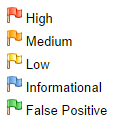
\includegraphics[scale=0.65]{images/alerts.png}
    \caption{Alert levels in \gls{zap}.}
    \label{fig:zapalerts}
\end{figure}


\subsection{Results Overview}
\label{sec:zapresult-overview}
\paragraph{}
Scanning \gls{dhis} with \gls{zap} revealed the following issues(shown in~\ref{fig:zapresults}):

\begin{figure}[h]
    \centering
    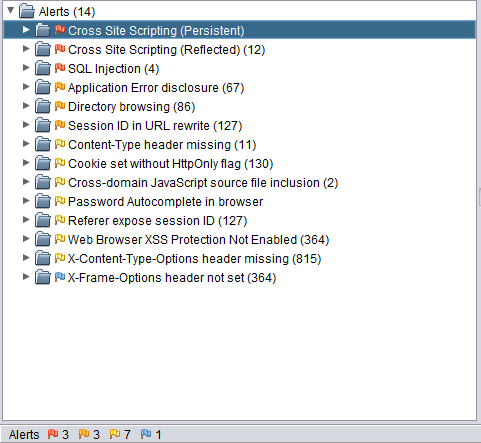
\includegraphics[scale=0.65]{images/zap-result.png}
    \caption{Result from \gls{zap}.}
    \label{fig:zapresults}
\end{figure}

\paragraph{}
One thing to note about the analysis, is that the amount of duplicated results are really high. 
Therefore the alert: "X-Content-Type-Options header missing" with 368 occurrences can be seen as one and the same alert. 
The rest of the report will be based on this observation, discussing classes of vulnerabilities instead of each occurrence, while taking examples from each when trying to determine a solution for the problem.
Looking at the results, the first thing that stands out is the large amount informational and low level security alerts, in contrast to the small amount of high level alerts.
This may indicate a certain level of focus towards well known security vulnerabilities by the developers.

\subsection{Results Inspected}
\paragraph{}
Ranking from lowest to highest alert level we will inspect each of the different vulnerabilities.

\subsubsection{X-Frame-Options header not set (Informational)}
\paragraph{}
This alert is pretty straight forward.
It only means that the \gls{http} response coming from the server should include the X-Frame-Options header to protect against 'Clickjacking'\cite{clickjacking} attacks.
Clickjacking is a form of hijacking attack, where the attacker hides malicious buttons or links on top the actual webpage.
Users is then tricked into clicking them instead of their intended target, thus hijacking there click.
The developers of the codebase doesn't seem to know about this potential exploit as every response from the server comes without this header.

\subsubsection{X-Content-Type-Options header missing (Low)}
\paragraph{}
As the previous issue mentioned, is this issue also about setting a header parameter.
However, in this case should the 'X-Content-Type-Options' be set to 'nosniff' \cite{no-sniff}. 
This stops older versions of Chrome and Internet Explorer from performing \gls{mime}-sniffing. 
\gls{mime}-sniffing is the browser trying to determine the MIME type of the current content. 
This is harmless as itself, but opens up to some security vulnerabilities by confusing the \gls{mime}-sniffing algorithm into interpreting the data the wrong way and not correctly assigning the content type.


\subsubsection{Web Browser \gls{xss} Protection Not Enabled (Low)}
\paragraph{}
This means that the browsers \gls{xss} filter is not enabled or manually disabled by setting a \gls{http} header parameter.
More about this and other common \gls{http} header parameters can be found here\cite{important-headers}. 

\subsubsection{Referrer expose session ID (Low)}
\paragraph{}
The analysis discovered multiple links leading away from the application and into an external host.
This in combination with having the session ID in the \gls{url}(will talk more about this later) can potentially be dangerous as the session ID may be disclosed in the 'referrer' header parameter in the request to the external host.
The 'referrer' parameter contains the \gls{url} where the request was coming from, meaning that the session ID is exposed inside the request.

\subsubsection{Password Autocomplete in browser (Low)}
\paragraph{}
The username and password is on autocomplete, which means that if an attacker gets access to your computer he can access the system using your credentials.

\subsubsection{Cookie set without HttpOnly flag (Low)}
\paragraph{}
Multiple cookies in the application does not contain the HttpOnly flag, which means that the cookies can be accessed using \gls{js}.
If an attacker manage to run a malicious script on the application, the cookies will be accessible and can be stolen.

\subsubsection{Content-Type header missing (Low)}
\paragraph{}
Some responses in the application doesn't set the Content-Type header.
Setting the Content-Type gives you the control over how the content will be handled by the browser.
In other words, the browser doesn't have to guess the content type and possibly make a mistake while doing so.

\subsubsection{Session ID in \gls{url} rewrite (Medium)}
\paragraph{}
The application stores the session ID in the \gls{url}, which as we discussed previously can be exposed through the referrer header parameter when accessing a different host from your application \cite{url-sessionid-risks}.

\subsubsection{Directory browsing (Medium)}
\paragraph{}
The analysis detected that it was possible to view the directory listing.
This may reveal backup source files and other hidden files which contains sensitive information.

\subsubsection{Application Error disclosure (Medium)}
\paragraph{}
It is possible that the application contains error messages which may disclose implementation details. 
In this case this alert is closely related to the previous section, as this alert is triggered by the fact that you can traverse the directory listing. 
The error may be a configuration problem or perhaps it only occurs because we are running the application locally.

\subsubsection{Cross-Site Scripting - Reflected (High)}
\paragraph{}
The last and only high level alert is a reflected \gls{xss} vulnerability. 
Reflected \gls{xss} means that the attack is not stored in the application itself, but rather in a URL or \gls{http} header parameter.
So it can only be triggered by a user which opens a maliciously crafted link or a third-party web page.
\gls{zap} managed to inject a small script on six different occasions when scanning the application.
The application used the \gls{url} as part of the application on several places, which is where it could be taken advantage of.
\gls{xss} attacks can be very harmful, and in a worst case scenario an attacker can hijack the users account information without the user having any idea what happened.
This is a very serious vulnerability and needs to be fixed as soon as possible.


\section{HP Fortify}
\label{sec:hpfortify}
\subsection{Approach}
\paragraph{}
As mentioned in Chapter~\ref{sectionfortifytool}, \gls{for} is an automated static analysis tool for exposing security vulnerabilities in software applications. 
The process of automated testing is an important part of securing software as they tend to find security issues that manual code reviews simply doesn't reveal.
Running the \gls{for} \gls{sca} scan on the entire codebase found over ten thousand security issues where over hundred of them were marked as critical.
In addition, does \gls{for} have some problems with analysing large amount of source code as it requires a whole lot of memory.
Therefore has the focus been narrowed to a smaller part of the codebase in order to provide a more comprehensive and complete analysis.

\subsection{Results Overview}
\paragraph{}
The \gls{sca} scan has primarily been limited to the module called dhis-web-mobile. In Eclipse you can right clicking the project and then clicking on analyse project to start the \gls{sca} scan.
During scan completion will the perspective change automatically to \gls{for} Audit perspective.
The result of the scan will shown up in this perspective, and in figure~\ref{fig:issuesfoundmobilemodule} you can see what the scan of the web-module revealed:

\begin{figure}[ht]
\RawFloats
    \begin{minipage}[b]{0.48\linewidth}
        \begin{itemize}
			\item Critical: 148
			\item High: 149
			\item Medium: 1
			\item Low: 405
		\end{itemize}
    \end{minipage}
    \hfill
    \begin{minipage}[b]{0.48\linewidth}
	    \centering
	    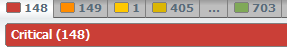
\includegraphics[scale=0.65]{images/foundissues.png}
	    \caption{\gls{for} \gls{sca} scan security vulnerabilities distribution between low, medium, high and critical. }
    	\label{fig:issuesfoundmobilemodule}
    \end{minipage}
\end{figure}

\paragraph{}
There might even be more issues within this module since the machine ran out of memory during the scan.
However, the further analysis will be based on the results from this scan.
Since the amount of issues found are so immense, can't all the found issues be taken care of. 
As a result will only particularly interesting issues be taken into account and a varied composition of issues to cover a greater base of issues.
In addition, will issues on the \gls{owasp} top 10 list be favoured over other issues and chosen from all the priority order ratings but mostly high and crucial.
As with the \gls{zap} scan does also this scan reveal a lot of duplicated issues and they will be considered the same issue.


\subsection{Results Inspected}
\subsubsection{Password Management: Hardcoded Password (Critical)}
\paragraph{}
It is never a good idea to hardcode a password.
It allows developers to view the password and makes it difficult to fix the problem. 
Once the code is in production a patch will be needed to fix the issue.
A good rule of thumb is to never hardcode passwords.
Storing passwords in plain text anywhere on the system allows anyone with sufficient permissions to read and potentially misuse the password.
The code presented in listing~\ref{hardcodedpassword} is found in DatabaseAutomaticAccessProvider class, revealing a hardcoded username and password.

\begin{lstlisting}[caption=Hardcoded username and password, label=hardcodedpassword]

	String username = "admin";
	String password = "district";
	
\end{lstlisting}


\subsubsection{Cross-Site Scripting: Reflected (Critical)}
\paragraph{}
A method sends invalidated data to a web browser which can result in execution of malicious code.
This kind of attack happen when data from an untrusted source enters an application where the untrusted source is a web request.
An untrusted source basically means every user of the application.
The data that is sent with the request is not being validated properly which makes it possible to execute scripts on the server or the database.
You should always validate data provided by an untrusted source.


\subsubsection{Shared Sink: Open Redirect (Critical)}
\paragraph{}
In RequiredLoginFilter is invalidated data sent to an \gls{http} redirect function. 
Redirects allow web application to redirect users to different pages either within the application or to external sources.
If user supplied data is part of the determining process of redirecting a user, then the data must be validated.
Attackers can utilize open redirects to trick users into visiting a \gls{url} to a trusted site and redirecting them to a malicious site.
Open redirects are often abused as part of phishing scams to harvest sensitive data.
You should not allow the end-user to control the destination in a redirect.

\subsubsection{Injection: Log Forging (High)}
\paragraph{}
Applications use log files to store a history of events or transactions for later review, statistics gathering, or debugging.
The method CreateAccount method in the AccountController class writes invalidated user input to the log.
A potential attacker could take advantages of this behaviour to forge log entries or inject malicious content into the log.
This is typically a vulnerability when data enters an application from an untrusted source and the data is written to an application or system file.


\subsubsection{Bad Practices: Dynamic Method Invocation (High)}
\paragraph{}
A translate action exposes a public method that can be invoked by end users overriding the actions execute method.
This is part of Apache Struts 2 framework which is an extensible framework for creating enterprise ready applications.
The framework streamline the full development cycle, all the way from building, to deploying and maintaining. 
Dynamic method invocation allow an action to expose methods other than execute.
The "!" character can be used in the \gls{url} to invoke any public method in the action if dynamic method invocation is enabled.
Developers that are not aware of this feature can inadvertently expose business logic. 

\subsubsection{System Information Leak: External (High)}
\paragraph{}
The method mapException catches an exception that might reveal system data or debugging information. 
The information could help an adversary form an attack plan.
When the exception is thrown, might data about the system be revealed. 
The revealed data can for example be information about the operating system, full pathnames, the existence of user names, or locations of configuration files, which could help an attacker plan an attack.
Too informatively error messages could tell attackers precisely what kind of attacks the application is vulnerable to.

\subsubsection{Password Management: Password in comment (Low)}
\paragraph{}
As mentioned earlier it is never a good idea to hardcode passwords. 
This can compromise system security in a way that cannot be easily remedied.
Storing password details within comments is equivalent to hardcoding passwords.
Once the code is published, the password is now leaked to the outside world and cannot be protected or changed without patching the software. 
This is the case in several files in the codebase, revealing password details in the comment.


\section{Chapter Closing Words}
\paragraph{}
In the next chapter (chapter~\ref{cha:part4}) we will try to look further into these problems, and look at how they can be solved, as well as give further advice on securing the web application.
The results from the two scans will also be compared and combined to make a complete evaluation of all the improvements that can be done.


\chapter{Analysis, Evaluation and Recommendations}
\label{cha:part3}

\textit{This chapter will combine the results from both \gls{zap} and \gls{for}, with the purpose of finding common flaws and vulnerabilities.}
\textit{We then discuss possible solutions and what we recommend to improve the system.}

\section{Solutions and Recommendations}
\subsection{Comparing the results}
%Combine the most critical result (XSS)
%Both Zap and Fortify found this
%Seems to be a big problem in the application
The tools used in this report \gls{zap} and \gls{for} found a lot of different vulnerabilities, ranging from low to critical severity.
The only overlapping vulnerability worth mentioning was reflected \gls{xss}.
The reason for this is its high level of severity and that it was discovered multiple times.
It was found with a live attack from \gls{zap} and the discovery of invalidated input from \gls{for}.
This section will therefore be focusing on how to better protect the system from \gls{xss}.
One problem with finding this type of flaw in an already deployed application is that to fully mitigate \gls{xss} you need to start at the design and architectural level.
Choosing the correct libraries and implementing them correctly is much easier to do early in development.
That being said it is off course possible to implement later, but it is much harder to cover the entire application in later stages.

\paragraph{}
There are many ways of preventing \gls{xss}, which depends on what framework you are using and how much control you want over it.
\gls{dhis} uses the spring framework, which allows you to escape unwanted input from the user.
You can specify this on three different levels in your application \cite{preventxss}:
\begin{itemize}
	\item Global level - in the web.xml file you can specify that all input should be checked for unwanted html or script tags. 
See Listing \ref{globallevel}.
	\item Page level - specify input escaping per page. 
See Listing \ref{pagelevel}
	\item Form level - specify input escaping on every attribute inside a html form, such as a text field.
See Listing \ref{formlevel}

\end{itemize}

\begin{lstlisting}[caption=Escape input in web.xml file, label=globallevel]

	<context-param>
		<param-name>defaultHtmlEscape</param-name>
		<param-value>true</param-value>
	</context-param>
	
\end{lstlisting}

\begin{lstlisting}[caption=Escape input on a page level, label=pagelevel]

	<spring:htmlEscape defaultHtmlEscape="true" />
		
\end{lstlisting}

\begin{lstlisting}[caption=Escape input on a specific input field, label=formlevel]

	 <form:input path="name" htmlEscape="true" />
	
\end{lstlisting}

The recommended approach to ensure the entire application is secure is off course applying it on a global level.

\paragraph{}
If you do not want to use the standard frameworks it is important to keep a few things in mind.
Assume that all input is compromised, and use an ''accept known good" input validation strategy.
In other words, use a whitelist of acceptable inputs.
You should also ensure that you perform input validation at well-defined interfaces in the application.
Doing so will ensure that even if a component is removed from the application it will still be protected.

\paragraph{}
As a final note we recommend that you read the OWASP \gls{xss} Prevention Cheatsheet\cite{cheatsheet} as it contain everything you will ever need to know about \gls{xss}. 

\subsection{\gls{zap}}

\subsubsection{Missing header parameters}
\paragraph{}
In \ref{cha:part2} we saw that the codebase contained several ''Missing header parameter" vulnerabilities, such as \textit{Content-Type} and 
\textit{X-Frame-Options}.
The solution for this type of flaws is easy to understand, since all you need to do is set the header parameter in you \gls{http} requests.
\gls{dhis} is using \gls{spring} as there server-side implementation, and the additional framework \gls{spring}-security.
\gls{spring}-security has all of these header parameters on by default so in theory it should work out of the box.
One thing that could be the problem is that on certain requests they are specifying a header in the code.
By doing so they are saying that only the specified header should be included.

\paragraph{}
Our recommendation is to review the code which handles request and response from the client and see if you are specifying any headers.
If so then you have to specify each header manually for that response.\cite{spring-security}

\subsubsection{Password Autocomplete in browser}
\paragraph{}
In many cases there isn't any need to disable password autocomplete, as you need access to the users computer in order to exploit this.
Nevertheless in some cases this might be necessary, and the way to disable autocomplete is quite easy as you can see in the example below.
\\
\textit{ \textless input type="password" name="foo" autocomplete="off" /\textgreater}

\subsubsection{Cookie set without HttpOnly flag}
\paragraph{}
By not setting the HttpOnly flag on your cookies you risk exposing them to malicious \gls{js}.
Fortunately there is two very easy ways to fix this if you are using \gls{java}, either programmatically(Listing \ref{httponly}) or declaratively by specifying it in the web.xml config file.\cite{httponly}
\\
\begin{lstlisting}[caption=Setting the HttpOnly Flag in Java,label=httponly]
Cookie cookie = getMyCookie("myCookieName");
cookie.setHttpOnly(true);
\end{lstlisting}


\subsubsection{Referrer expose session ID}
\paragraph{}
This is a consequential error caused by the application storing the session ID in the \gls{url}.
We will discuss how to solve this in section: \nameref{subsec:sessionid}.

\subsubsection{Session ID in \gls{url} rewrite}
\label{subsec:sessionid}
\paragraph{}
Storing the session ID solely in the \gls{url} is very dangerous as it is easy to hijack it.
It is recommended that you use a combination between storing it as a cookie and the \gls{url}.
Because cookies provide multiple security features such as the ''secure" attribute which instructs the browser to only send it through secure channels.
This stops any man-in-the-middle attacks trying to steal the session.\cite{session-management}

\subsubsection{Directory browsing}
\paragraph{}
As discussed in chapter \ref{cha:part2} this could be a false positive, since the application has been tested on a local machine.
Therefore it is hard to know if this even is a problem when deployed to a real web-server. 
To be safe it can be wise to try and browse the directory of a deployed application to see if this is possible.
If you discover that this is in fact possible, you need to access your .htaccess file which stores this kinds of policies and add the line:
\\
\textit{Options -Indexes} to it.
Doing so will turn of directory browsing in your application.

\subsubsection{Application Error disclosure}
\paragraph{}
This is an error which is caused by the fact that you can browse the directory of the application, as all the alerts came from those pages.
Therefore by solving the Directory browsing problem you will also solve this one.

\subsection{\gls{for}}
\paragraph{}
In this section will a solution to the problems mentioned in Section~\ref{sec:hpfortify} be provided.
Some of the problems have already been discussed, and will therefore be excluded in this section(\gls{xss} related issues). 

\subsubsection{Password Management: Hardcoded Password}
\label{passwordmanagement}
\paragraph{}
As mentioned, it is never a good idea to hardcode a password for a number of reasons.
Passwords should never be hardcoded and should generally be obfuscated and managed in external sources. 
The solution is simple, remove the hardcoded password from the source code and retrieve the password another way, e.g from a database.

\subsubsection{Shared Sink: Open Redirect}
\paragraph{}
Redirects allow web applications to direct users to different pages within the application or to external sites. 
\gls{for} claims that invalidated data is passed to a \gls{http} redirect function.
However, the invalidated data is not user created and it is therefore not necessary to validate the data.
Meaning that this a false positive problem found by \gls{for}. 

\subsubsection{Injection: Log Forging}
\paragraph{}
Log files are used to store history of application events for later review, statistics gathering, or debugging.
In listing~\ref{lstlogforging}, this is the case.
The variable inviteUserName is a request parameter from method invocation. 
Checking that the variable is not null and not empty is the only type of validation that is done. 
One way of prevent log forging is with indirection.
A set of legitimate log entries must be created that correspond to different logging events and only entries from this set can be logged.
This ensures that only a certain set of logging entries will occur in the logging file and additionally makes it easier to read the file.

\begin{lstlisting}[caption=Log forging in the AccountController class, label=lstlogforging]
	
	boolean invitedByEmail = (inviteUsername != null && !inviteUsername.isEmpty());

	log.info( "AccountController: inviteUsername = " + inviteUsername );


\end{lstlisting}

\subsubsection{Bad Practices: Dynamic Method Invocation}
\paragraph{}
The application fails to disable dynamic method invocation for struts 2.
As a developer using struts 2 you need to be aware of this, or else you can inadvertently expose business logic.
In order to prevent this, you must disable the function in the Apache Struts 2 framework.
This can be done multiple ways, one of them is to edit the struts 2 configuration file by adding this line:
\begin{center}
	\textit{\textless name="struts.enable.DynamicMethodInvocation" value="false" /\textgreater }

\end{center}


\subsubsection{System Information Leak: External}
\paragraph{}
You should always write error messages with security in mind.
In listing~\ref{lstsysteminformationleak}, the detail message string of the exception is written to the response object.
In production environments, turn off detailed error information in favour of brief messages.
Even brief error messages that do no reveal stack trace or database dumps can potentially aid an attacker. 
For example, an ''Access Denied" message can reveal that a file or user exists on the system.

\begin{lstlisting}[caption=Parts of the method mapException, label=lstsysteminformationleak]
	
	response.getWriter().write( exception.getMessage() );

	
\end{lstlisting}

\subsubsection{Password Management: Password in comment}
\paragraph{}
Passwords should never be hardcoded, not even in comments.
The solution proposed in Section~\ref{passwordmanagement} will be sufficient.


\section{Chapter closing words}
% Our opinion of zap and fortify
% How the results have been ? 

\subsection{The result}
\paragraph{}
With help from \gls{zap} and \gls{for} we have managed to reveal multiple vulnerabilities within the provided codebase, \gls{dhis}.
The scans revealed surprisingly many weaknesses, considering the calibre of the application.
The application is used as health management information system in a whole lot of countries and are being trusted to keep a lot of sensitive data safe and secure.
However, it doesn't necessarily mean that companies using the system is exposed to all these attacks because they most likely have their own security policies and security mechanisms wrapped around the application. 
Many vulnerabilities found that is marked as critical, requires an extreme skill in computing in order to even find the vulnerability at all, and then an even greater skill to exploit the vulnerability.
When the number of vulnerabilities found are that great in number, it should be kind of alarming and concerning.
Although, a very high number of the faults found are false positives and many of them are duplicated errors.



\subsection{Our opinion}
\paragraph{}
Writing this report has given us a lots of relevant experience in regards of working with security as well as exercise in writing reports.
Many relevant security related tools have been tried out and it has given us a great start with security oriented software development.
The writing of the report has been useful since it is highly relevant considering the writing of the masters thesis that lies ahead of us.
It will also give us a smoother transition when we now are heading into the writing of the thesis.
The course it self has thought us the importance of integrating security as early as possible in to development cycle.
In addition, we are now aware of all the different type of attacks that we need to pay attention to.
Not just how to protect against attacks, but also how to cope with eventual data compromise. 

\paragraph{}
% Overall opinion on the codebase as it is.





\newpage


\bibliographystyle{plain}
\bibliography{biblio}

\end{document}

